\section{The application of the animal model} \label{app:am}
In this appendix we give details on the application of the animal model to the simulated data. We have applied a univariate animal model, using the temporal trends in BLUPs (best linear unbiased predictors) to decompose changes in $\overline z$ into underlying processes.

\subsection{Animal model using the BLUPs approach} \label{app:am:blup}
Following \cite{Hadfield2010b}, we estimated the temporal change in the mean components of variation (breeding values, maternal effects, individual repeatability and within individual residual variation) by regressing their estimates on time, within a Bayesian framework. 
To this end we fitted a univariate animal model on the vector of size observations, $\boldsymbol{z}$, as:

\begin{equation}
\boldsymbol{z}=\boldsymbol{X_z}\boldsymbol{b_z}+\boldsymbol{D_1a}+\boldsymbol{D_2m}+\boldsymbol{D_3p}+\boldsymbol{D_4y}+\boldsymbol{Ir} \text{ .}\\
\end{equation}

\noindent Here $\boldsymbol{X_z}$, $\boldsymbol{D_1}$, $\boldsymbol{D_2}$, $\boldsymbol{D_3}$, $\boldsymbol{D_4}$ and $\boldsymbol{I}$ are design matrices, $\boldsymbol{b_z}$ is a matrix of fixed effects, $\boldsymbol{a}$, $\boldsymbol{m}$, $\boldsymbol{p}$ and $\boldsymbol{y}$ random effects accounting for the variance associated with breeding value, mothers, permanent environment and years respectively, and $\boldsymbol{r}$ represents residuals. The fixed part of the model included an intercept and the effect of age (up to second order). In addition to a random additive genetic effect, the model thus included three additional random effects: the identity of individual (accounting for any permanent environment effects), the identity of the mother and the year of measurement \parencite{Kruuk2004}.

From this model, the posterior distribution of each Best Linear Unbiased Predictors (BLUPs), that is the value of each level of the random effect, of the random effect $\boldsymbol{a}$, $\boldsymbol{m}$, $\boldsymbol{p}$ and $\boldsymbol{r}$ were extracted. 
Each posterior sample, $j$, of the BLUPs was regressed on time. For instance, for breeding values:
\begin{equation}
a_{i,j} = \mu_{a,j} + \bar{t_i} \beta_{a,j} + \epsilon_{i,j} \text{ ,}
\end{equation}
where $a_{i,j}$ is the posterior sample $j$ of the breeding value of the individual $i$, $\mu_{a,j}$ is the intercept for the $j$th regression, $\bar{t_i}$ is the mean time of presence of the individual $i$,  $\beta_{a,j}$ is the slope of the $j$th regression and  $\epsilon_{i,j}$ is the error. 
Combining all the slope estimates, $\beta_{a,j}$ we thus obtained the posterior distribution of the rate of change in the random effect \parencite{Hadfield2010b}.

\subsection{Alternative modelling of maternal effects}\label{app:am:newres}
The AM described above does not match the simulation process on maternal effects. Indeed, in our simulations, offspring size at birth is influenced by the current size of their mothers (in an additive, proportional way). The effect of a given mother on her offspring size therefore changes through her life. In contrast, the AM models maternal effects as a random intercept on mother identity, which assumes that a given mother influences her offspring size by a fixed propensity  throughout her life.
Various formulations of maternal effects in quantitative genetic models are for instance compared in \cite{Mcglothlin2014}. In this section, we present results from an AM that models maternal effects in a way that is more in agreement with the simulations process: maternal effects are modelled by including maternal size as a covariate, rather than maternal identity as a random effect.

Compared to the results of the AM in the main text, this alternative AM formulation estimated a less negative contribution of genetic evolution to trait dynamics, and a more negative contribution of maternal effects (Fig. B.1 shows the results of the two different AM for the scenario \sh). In the other scenarios a similar effect was obtained by changing the model specification (results not shown).

The negative contribution of maternal effects makes sense in our simulations, because maternal effects are modelled by adding up 10\% of mother size to the offspring birth size, and because mean size decreases with time (Fig. 1b). As a result, the effect of mother size on offspring birth size decreases with time. 
The scenario \sh did not include selection on size and no directional genetic change was therefore expected. However, the AM estimated on average a negative contribution of evolution when maternal effects were modelled as maternal identity. 
This bias is divided by two when maternal effects are modelled in the same way as they were simulated. The reason why the bias does not entirely disappear probably has to do with the fact that the maternal effects we have simulated are heritable (because they are proportional to size, which is itself heritable). As such, a model matching our simulation process should also account for genetic maternal effects\textemdash in addition to phenotypic maternal effects\textemdash \parencite{Mcglothlin2014} in order to fully disentangle the change in breeding values for size from the change in maternal effects.

\begin{figure}[ht]
\centering
	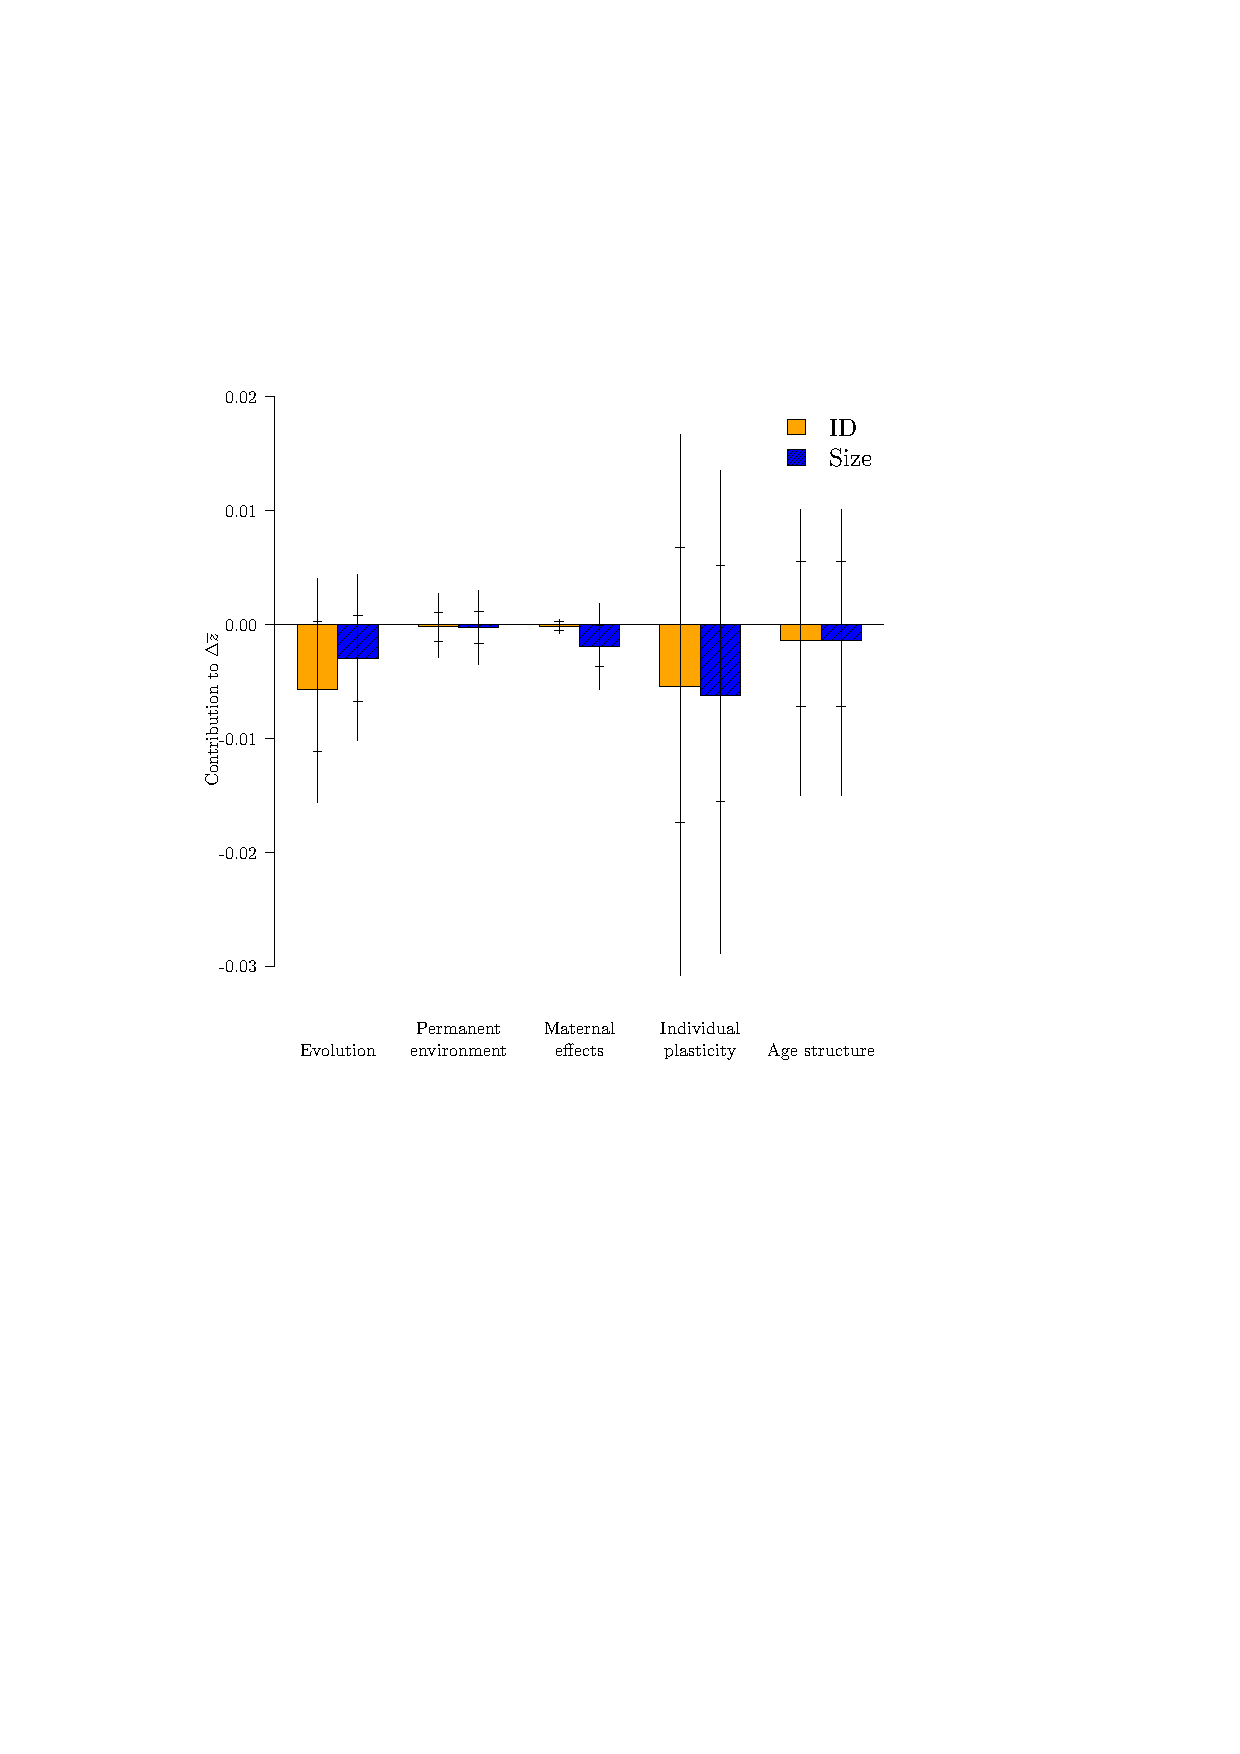
\includegraphics[width=0.8\textwidth]{Appendices/FigS3}
    \caption{\footnotesize Results of two animal models, either modelling maternal effects by fitting mother identity as a random intercept (yellow plain bars), or by fitting the size of the mother at birth of the focal individual as a continuous covariate (blue stripped bars). The latter model is closer to the process of data simulations, and provides a less biased estimation of genetic change (the expectation is zero for both models). Error bars represent the range in which 68\% (error bars until horizontal lines) and 95\% (entire error bars) of the contributions lie when applied to 100 replicates of the scenario \sh.}
    \label{app:AM:IDvsSize}
\end{figure}